The description of the analysis where were pefromed during the
research and helped to achieve the objective of the research.

\section{Stastical Hypothesis Testing}
The following independent unpaired stastical testing was peformed using 
IBM SPSS software. The ${H_o}$(null hypothesis) = there is no difference in 
predicting the class of pigmented skin lesions by automated system and 
medical professional. On the otherhand ${H_1}$(alternative hypothesis) = there is 
a difference in time required to predict pigmented skin lesions.
\begin{figure}[!htp]
    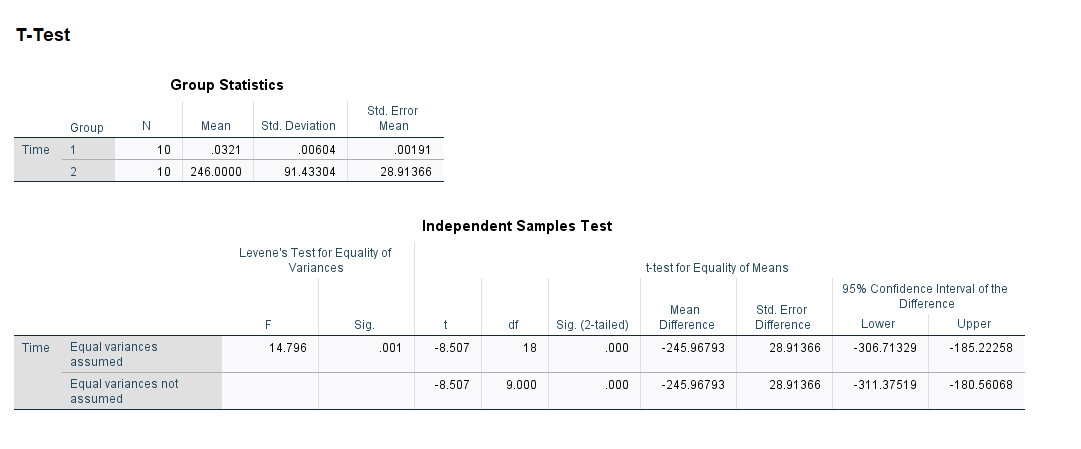
\includegraphics[width=15cm]{Images/ttest.png}
    \caption{Independent sample t-test}
    \label{fig:istt}
\end{figure}

The figure \ref{fig:istt} shows the results obtained by comparing the 
means of the time required by the automated system and medical professional to predict pigmented skin 
lesions. The group 1 in the test is reffered to the automated system and 
group 2 is reffered to medical professionals. Based on the p value obatined from the 
test which is 0.000 as in \ref{fig:istt} in the Sig(2-tailed) the null 
hypothesis is failed. Thus, it can be concluded that there is a significant 
difference in time required to peform diagnosis. The purposed automated machine 
is more time efficient to predict.

\section{Confusion Matrix}
\begin{figure}[!htp]
    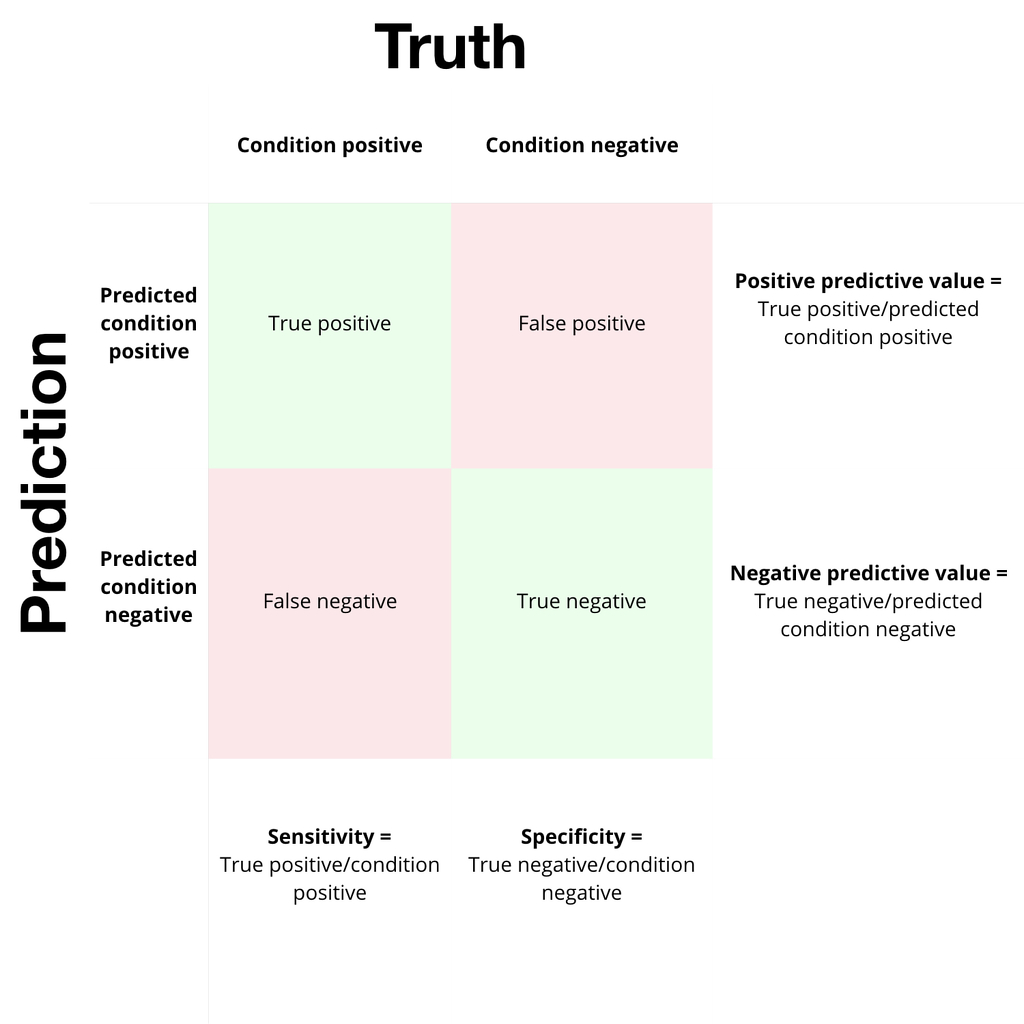
\includegraphics[width=\textwidth]{Images/cm.png}
\end{figure}
Confusion Matrix also known as the error matrix is the table to describe the 
perofarmance of automated system given true values of classification classes \citep{geekforgeeks}. The 
confusion matrix also allows the misclassified predicted labels by the automated 
and helps to evaluate the performance measures \citep{geekforgeeks}.

\subsection{Recall and Precision of Automated System}
\begin{center}
    Recall = ${ \frac{True Positive} {False Negative + True Positive}}$
\end{center}

\begin{center}
    Precision = ${ \frac{True Positive} {True Positive + False Positive}}$
\end{center}

The equations above are be used to obtain the precision and recall values of the 
convolutional neural network. The Precision and recall values are further used 
to compute the f-measures also known as the f1score to evaluate the performance of 
automated system. \\ 
\begin{center}
    F-measure = ${\frac{2 * Recall * Precision}{Recall + Precision}}$
\end{center}

\subsection{Confusion Matrix and F-measure of the Neural network}
\begin{figure}[!htp]
    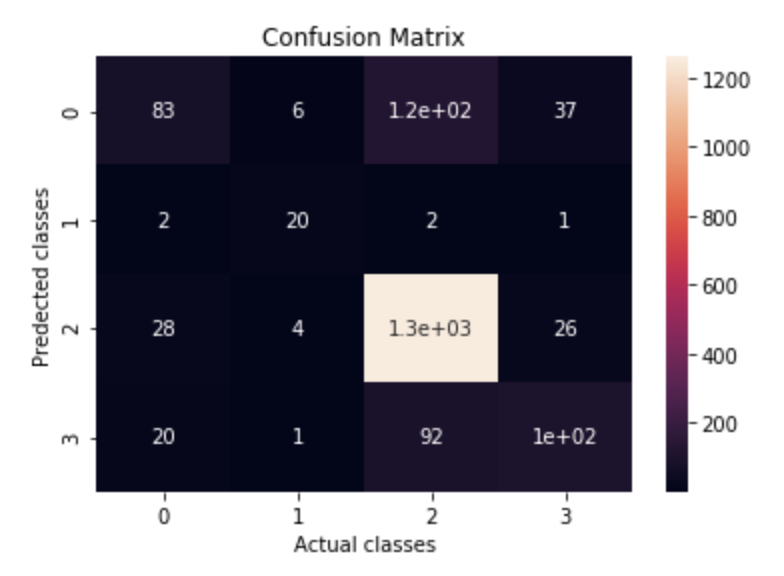
\includegraphics[width=\textwidth]{Images/cma.png}
    \caption{Error Matrix}
    \label{fig:ErrorMatrix}
\end{figure}

The confusion matrix was computed using the sklearn learn library which requires the predicted values and 
actual true labels for each pigmented skin lesions. Futhermore the confusion matrix  was plotted using heatmaps
in the matplotlib visualisation library.
\pagebreak

\begin{figure}[!htp]
    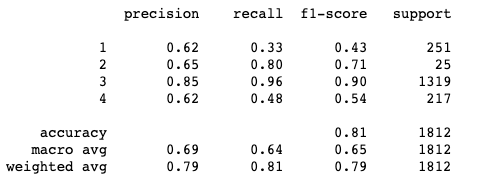
\includegraphics[width=\textwidth]{Images/f11.png}
    \caption{Classification Report of automated system}
    \label{fig:f11}
\end{figure}

\pagebreak

\section{Classification Comparison with participants}